\documentclass[twoside, letterpaper, 12pt]{report}
\usepackage{orthodoxservicebook}

\title{The Sunday Reader's Service of the \\ \textsc{Typica} \\ 2020 May 31}
\titlepic{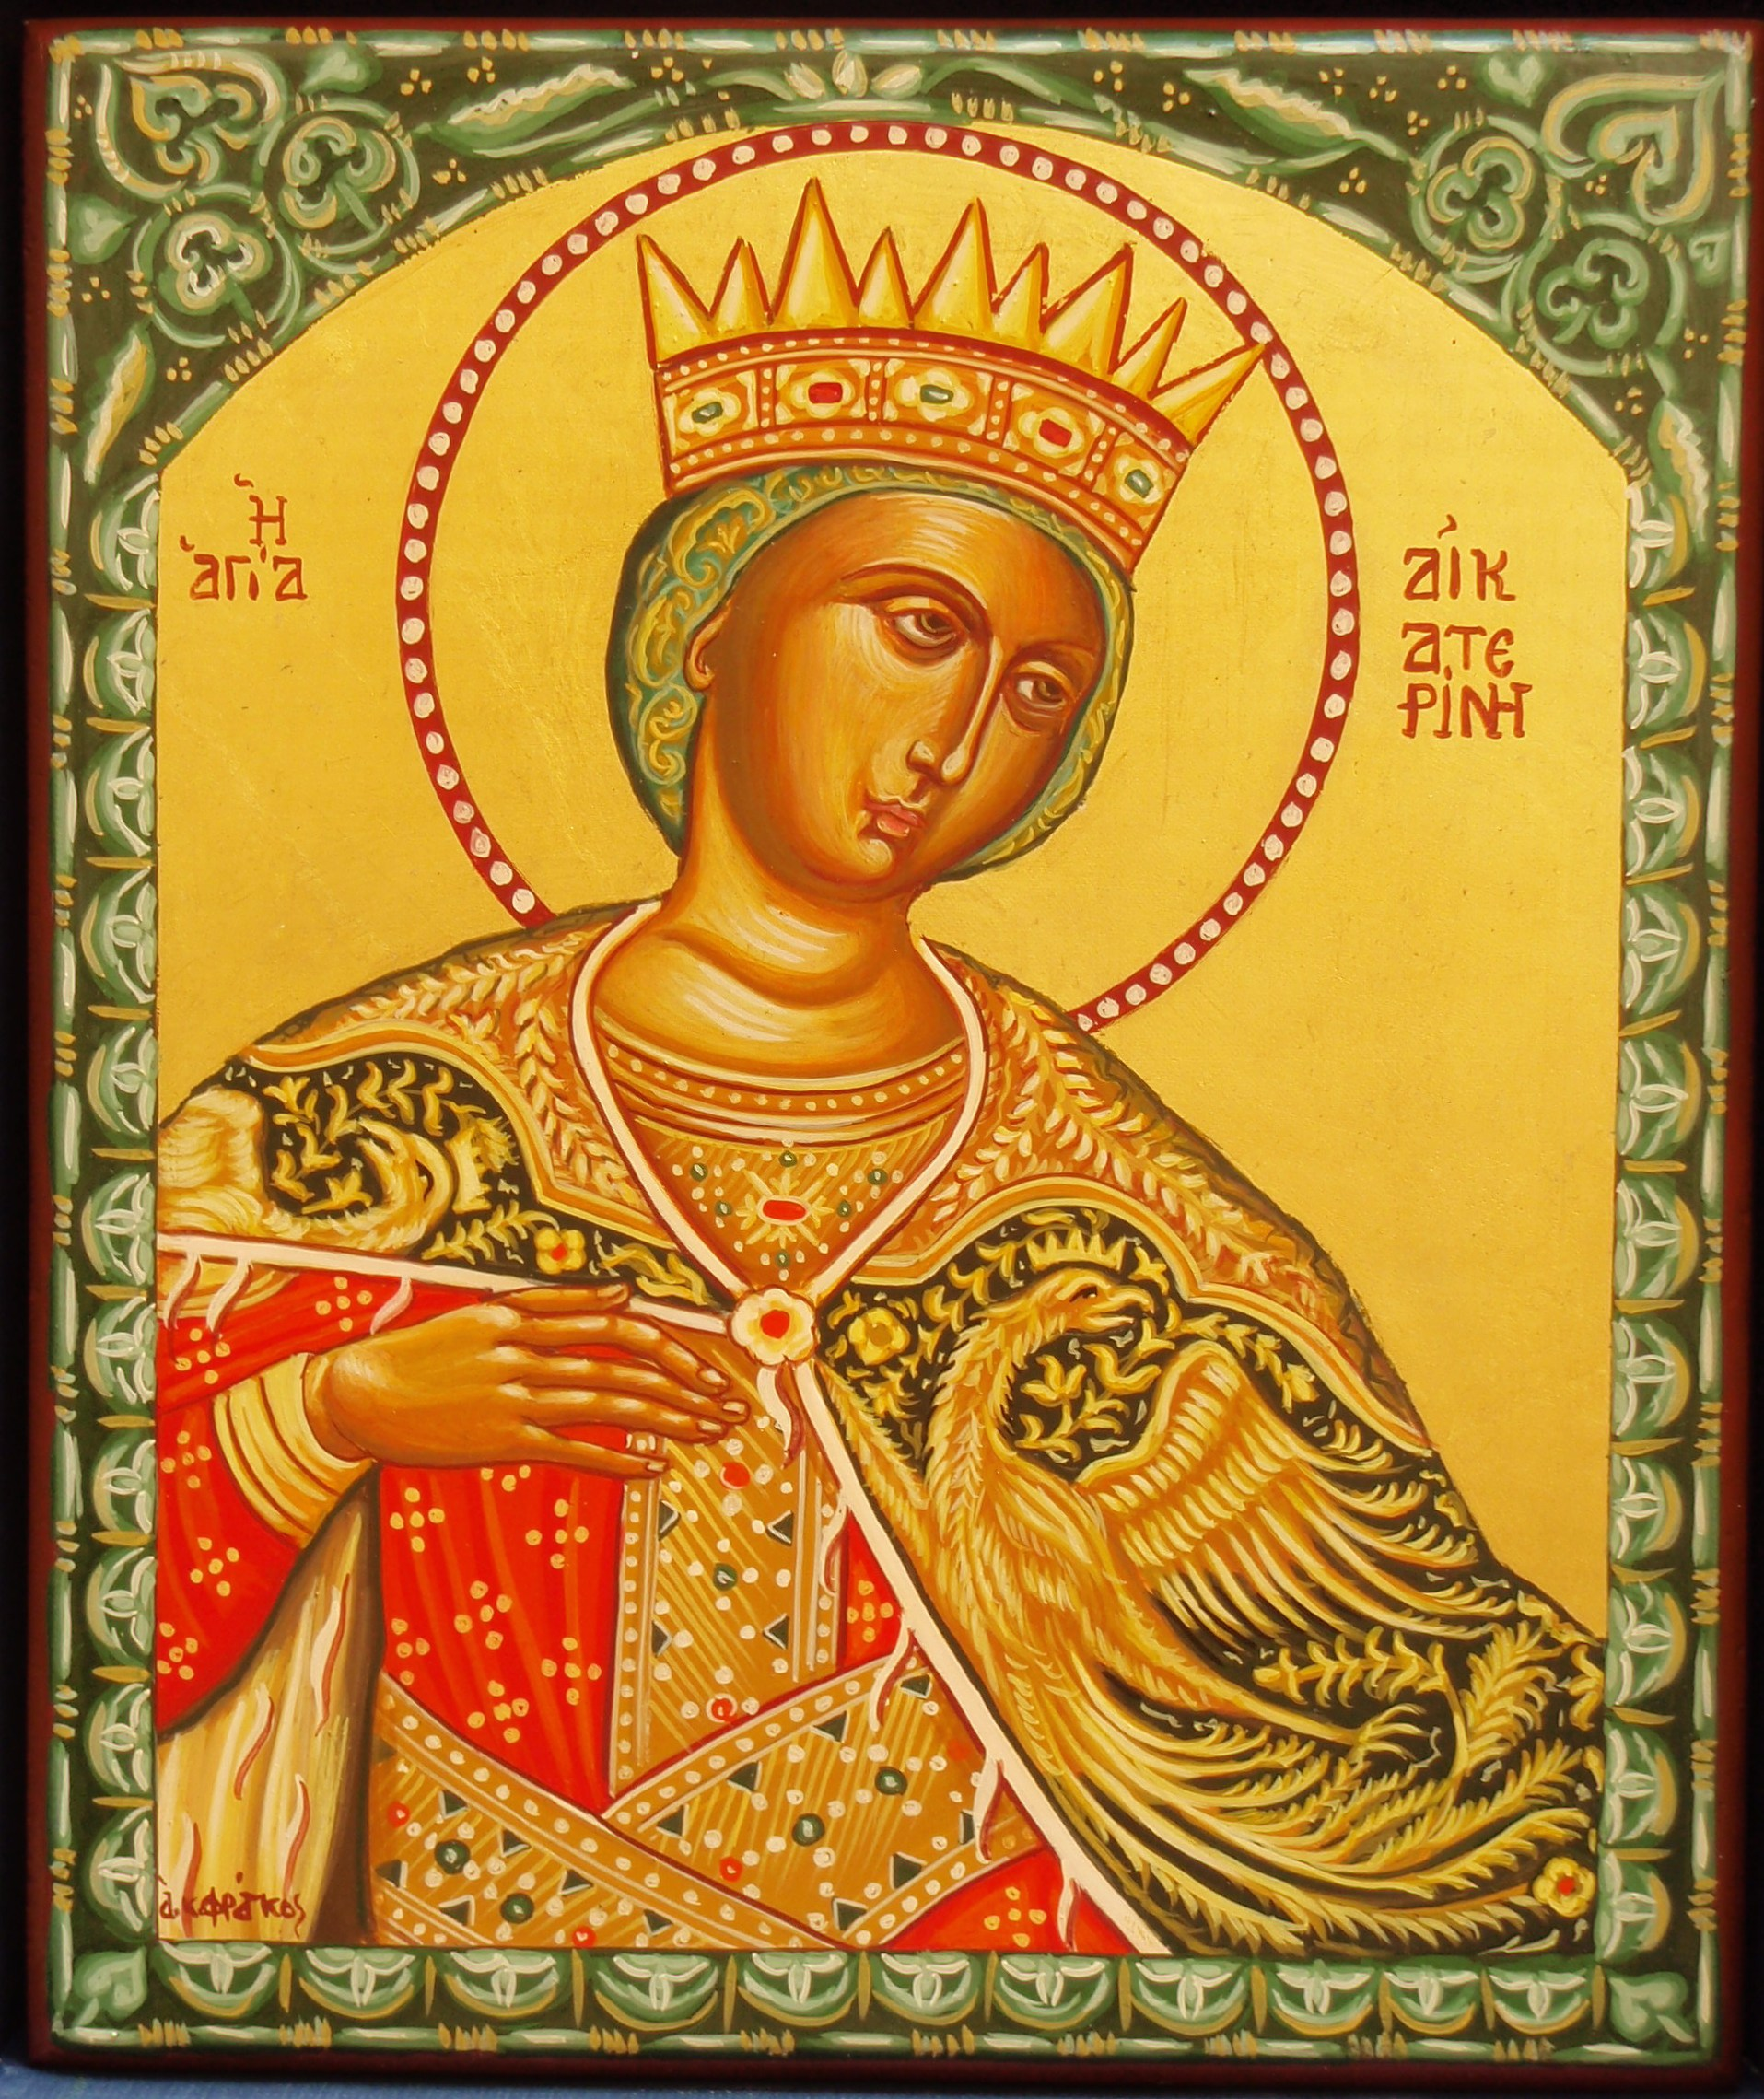
\includegraphics[width=0.5\textwidth]{Katherine1.jpg}}
\date{}
\author{}

\begin{document}
\maketitle
\pagestyle{empty} % Don't show page numbers
\instruction{This page intentionally left blank}
\cleardoublepage
\pagestyle{plain}
\setcounter{page}{1} % Set the page counter to 1 on the first real page
\chapter*{Service of Typica on Sunday, May 31}
\instruction{Sunday of the After-Feast of the Ascension\\
Commemoration of the Holy Fathers of the First Ecumenical Council}

\readerline{\throughtheprayers{}}
\choralresponse{./Z-Responses/Obikhod/Amen.ly}

\trisagionNeedsAmen[reader][prepentecost]

\choralresponse{./Z-Responses/Obikhod/Amen.ly}


\centeredsection{The First Antiphon}
\lilypondfile{./Liturgy/B-FirstAntiphon/BlessTheLord_Greek-Music.ly}

\centeredsection{The Second Antiphon}
\lilypondfile{./Liturgy/C-SecondAntiphon/PraiseTheLord_Greek-Music.ly}

\centeredsection{The Third Antiphon}
\lilypondfile{./Liturgy/D-ThirdAntiphon/Beatitudes_Moscow-Music.ly}

\centeredsection{The Epistle}

\instruction{Both of the New Testament lessons are read
without liturgical introduction or conclusion.
The readers start with “The Reading from…” and proceeds}

\paragraph{The Reading from the Acts of the Apostles. (20:16-18, 28-36)}\mbox{}\\

\begin{maybetwocolumns}
  In those days, Paul had decided to sail past Ephesus, so that he might not have to spend
  time in Asia; for he was hastening to be at Jerusalem, if possible, on the day of Pentecost. And
  from Miletus he sent to Ephesus and called to him the elders of the church. And when they came
  to him, he said to them: “Take heed to yourselves and to all the flock, in which the Holy Spirit has
  made you overseers, to care for the church of God which he obtained with the blood of his own
  Son. I know that after my departure fierce wolves will come in among you, not sparing the flock;
  and from among your own selves will arise men speaking perverse things, to draw away the
  disciples after them. Therefore, be alert, remembering that for three years I did not cease night or
  day to admonish everyone with tears. And now I commend you to God and to the word of His
  grace, which is able to build you up and to give you the inheritance among all those who are
  sanctified. I coveted no one’s silver or gold or apparel. You yourselves know that these hands
  ministered to my necessities, and to those who were with me. In all things I have shown you that
  by so toiling one must help the weak, remembering the words of the Lord Jesus, how He said, ‘It
  is more blessed to give than to receive.’” And when he had spoken thus, he knelt down and prayed
  with them all.
\end{maybetwocolumns}

\centeredsection{The Gospel}

\instruction{Both of the New Testament lessons are read
without liturgical introduction or conclusion.
The readers start with “The Reading from…” and proceeds}

\paragraph{The Reading from the Holy Gospel according to St. John. (17:1-13)}\mbox{}\\

\begin{maybetwocolumns}
  At that time, Jesus lifted up His eyes to heaven and said, “Father, the hour has come; glorify
  Thy Son that the Son may glorify Thee, since Thou hast given Him power over all flesh, to give
  eternal life to all whom Thou hast given Him. And this is eternal life, that they know Thee the
  only true God, and Jesus Christ Whom Thou hast sent. I glorified Thee on earth, having
  accomplished the work which Thou gavest Me to do; and now, Father, glorify Thou Me in Thy
  own presence with the glory which I had with Thee before the world was made. I have manifested
  Thy Name to the men whom Thou gavest Me out of the world; Thine they were, and Thou gavest
  them to Me, and they have kept Thy word. Now they know that everything that Thou hast given
  Me is from Thee; for I have given them the words which Thou gavest Me, and they have received
  them and know in truth that I came from Thee; and they have believed that Thou didst send Me. I
  am praying for them; I am not praying for the world but for those whom Thou hast given Me, for
  they are Thine; all Mine are Thine, and Thine are Mine, and I am glorified in them. And now I
  am no more in the world, but they are in the world, and I am coming to Thee. Holy Father, keep
  them in Thy Name, which Thou hast given Me, that they may be one, even as We are one. While
  I was with them, I kept them in Thy Name, which Thou have given Me; I have guarded them, and
  none of them is lost but the son of perdition, that the scripture might be fulfilled. But now I am
  coming to Thee; and these things I speak in the world, that they may have My joy fulfilled in
  themselves.”
\end{maybetwocolumns}

\centeredsection{Troparia Before the Creed}
\instruction{Plain reading}
\begin{reader}
\item[Reader 1:] The heavenly choir singeth thy praises, saying:
  Holy, holy, holy, Lord of Sabaoth; heaven and earth are full of Thy glory.

\item[Reader 2:] \emph{Come unto him, and be enlightened,
               and your faces shall not be ashamed.}
  The heavenly choir singeth thy praises, saying:
  Holy, holy, holy, Lord of Sabaoth; heaven and earth are full of Thy glory.

\item[Reader 1:] \emph{\glory}
  The choir of the holy angels and archangels,
  with all the powers of heaven, singeth thy praises, saying:
  Holy, holy, holy, Lord of Sabaoth; heaven and earth are full of Thy glory.

\item[Reader 2:]\emph{\nowandever}
\end{reader}

\centeredsection{The Creed}
\input{Common/TheCreed.txt}


\centeredsection{Prayer of Forgiveness}
\readerline{Forgive, remit, pardon, O God, our sins,
  both voluntary and involuntary, in deed and in word, in knowledge or in ignorance,
  committed by night or by day, in mind and in thought.
  Forgive us them all, for thou art good and lovest mankind.
}


\centeredsection{The Lord’s Prayer}
\input{Common/LordsPrayer.txt}

\readerline{Through the prayers of our holy fathers, Lord Jesus Christ our God, have mercy on us.}
\choralresponse{./Z-Responses/Obikhod/Amen.ly}


\centeredsection{Kontakia for Pascha in Tone 6}
\lilypondfile{./Pentecostarion/Ascension/Ascension-Kontakion-T6-Byz-Karam-Music.ly}

\readerline{\lhmForty}

\readerline{
  O Christ our God, Who art worshipped and glorified at all times at every hour both in
  heaven and on earth; Who art long-suffering and plenteous in mercy and compassion; Who lovest
  the just man and showest mercy upon the sinner; and Who callest all men to repentance through 
  the promise of blessings to come; receive, O Lord, at this very hour our supplications, and direct
  our lives in the way of Thy commandments: sanctify our souls, purify our bodies, set our minds
  aright, cleanse our thoughts; deliver us from all affliction, trouble, and distress; compass us about
  with Thy holy angels, that, guided and guarded by them, we may attain unto the unity of the Faith,
  and to the knowledge of Thine unapproachable glory; for Thou art blessed unto ages of ages. Amen.
}

\begin{reader}
  \item \lhmThree{}\\\emph{\gne{}}
  \item \morehonorablethanthetherubim{}
  \item \throughtheprayers{}
\end{reader}

\begin{maybetwocolumns}
\choralresponse{./Z-Responses/Obikhod/Amen.ly}

\readerline{\blessedbethename{}\thrice{}}

\centeredsection{Psalm 33}
\input{./Psalms/Psalm033-unknowntrans.txt}

\end{maybetwocolumns}

\peopleline{\gne}


\centeredsection{A Homily}
\begin{maybetwocolumns}
\instruction{Ascending with Christ into Heavenly, Not Earthly, Glory:\\
Homily for the Sunday after the Ascension and Commemoration of the Holy Fathers of the
First Ecumenical Council of Nicaea in the Orthodox Church\\
Fr. Philip LeMasters, pastor, St. Luke Antiochian Orthodox Church of Abilene, Texas}

Forty days after His glorious resurrection, our Lord, God, and Savior Jesus Christ ascended
in glory into heaven and sat at the right hand of God the Father. He did so as One Who is fully
divine and fully human, One Person with two natures. He ascended with His glorified, resurrected
body which still bore the wounds of His crucifixion. The Ascension shows that through Him our
humanity has come to participate by grace in the eternal life of the Holy Trinity. He has made us
“partakers of the divine nature” who may share in His fulfillment of what it means to be a human
person in God’s image and likeness.

Today we commemorate the Holy Fathers of the First Ecumenical Council in Nicaea. They
rejected the teaching of Arius that Jesus Christ was not truly divine, but a kind of lesser god created
by the Father at a certain point. The Council declared, as we confess to this day in the Nicene
Creed, that our Savior is “the Son of God, the only-begotten, begotten of the Father before all
worlds. Light of Light, very God of very God, begotten, not made, of one essence with the Father,
by Whom all things were made.” The Fathers of Nicaea saw clearly that the One Who brought us
into the eternal life of God must Himself be eternal and divine. Only God could make human
persons “partakers of the divine nature” by grace.

Had Christ been merely a creature or an especially impressive religious teacher or example, He
would have remained captive to the corruptions of the world as we know it. He could have taught
and inspired people, but would not have been able to conquer death or make a path for us to find
the fulfillment of our humanity in the Holy Trinity. Those who water down the faith to the point
of viewing the Savior as simply an excellent human being make it impossible to acknowledge
Christ as the One Who has truly united humanity and divinity in Himself. We can learn a lot from
great teachers and examples, but only the Son of God can make us participants in life eternal. Only
He could say to the Father, “Glorify Me in Your own presence with the glory which I had with
You before the world was made.”

The divine glory displayed in Christ’s ascension is entirely different from the power and fame that
people find so appealing in our world of corruption. At some level, we all know how weak and
insignificant we are in the larger scheme of things. That is why we so easily make false gods of
just about anything that can distract us from recognizing the truth about ourselves, including the
inevitability of death. Putting our ultimate trust in nations, rulers, and riches—or our health,
appearance, talents, and relationships–or any created thing leads inevitably to idolatry, for it is a
form of worshiping a false god, regardless of whether we call it a religion. Doing so will also lead
us to demonize our enemies, real and imagined, because it often makes us feel better about
ourselves by comparison when we have someone else to condemn. That is surely one of the
reasons that so many people in our culture have become slaves to anger and hatred toward those
they view as their rivals or opponents in a zero-sum game for getting all the glory by being on the
right side.

The glory of our ascended Lord is the complete opposite of such pathetic and perverse efforts to
build ourselves up at the expense of others. Remember that He ascended only after descending,
only after dying on the Cross, being buried in a tomb, and descending into Hades. He rose from
the dead because He had humbled Himself to the point of accepting rejection, torture, and
crucifixion as a blasphemer and a traitor. He was mocked as a failure and made a public example
of what happened to people who dared to challenge the authority of Rome, even though His
Kingdom is clearly not of this world. He completely repudiated earthly glory in order to make a
way for us into the brilliant joy of heaven.

Christ endured all this, not simply as a religious teacher or virtuous person, but truly as the eternal
Son of God Who spoke the universe into existence. Let that sink in for a moment, for the
unfathomable humility of the Savior destroys our usual assumptions about what it means to be
high and mighty. The divine glory revealed so powerfully at His ascension shines brilliantly in
contrast to what passes for honor in a world that typically chooses to remain in the dark night of
the tomb. If we dare to identify ourselves with Him, we must open the eyes of our souls to the
light of His heavenly glory and refuse to wander in spiritual blindness. In order to celebrate the
Ascension with integrity, we must ascend with Him into the eternal life of the Holy Trinity even
as we live and breathe with our bodies in a world that remains very far from the fullness of His
Kingdom.

By rising into heavenly glory as the God-Man, He has shared His gracious divine energies with
us. He shows us what it means to be truly human in the divine image and likeness. In order to
unite ourselves to Him, we must reorient our desires for fulfillment, meaning, and joy to the One
Who overcame the worst the darkened world could do in order make us participants in the eternal
day of His heavenly reign. The contrast between the heights of heaven and the mundane realities
of our lives is obviously very great. The point of division is not, however, that we are ordinary
people with common problems who belong to a very small parish. It is, instead, that we have not
united ourselves to Christ in holiness to the point that every dimension of our life in this world has
become a brilliant icon of His salvation.

Of course, that is a very high goal which no one may claim to have fulfilled. God is infinitely holy
and the journey to become perfect as our Father in heaven is perfect is truly eternal. No matter
where we are on that path, we must all ask our ourselves quite seriously whether we are ascending
with Him into greater holiness as we go through our daily lives, face whatever set of challenges
we have, and respond to the constant barrage of temptations to put our trust elsewhere. It may be
easy to attend services, sing in praise of the Ascension, and call ourselves Christians, but it is much
more demanding to conform ourselves to Christ such that His radiant glory shines through us.

We should not dream of performing grand gestures of holiness, for that would likely lead us into
prideful fantasies. Instead, we do well to focus on taking the small steps that we are capable of
right now in relation to the people around us and the circumstances with which we are familiar.
That means humbling ourselves to put the needs of others before our own preferences in our
families, friendships, and workplaces, as well as in our parish.

Christ prayed to the Father that His followers “may be one, even as We are one.” We will never
ascend in holiness if we think that we relate to God as isolated individuals with a religion that
concerns only what we do when we are alone. The Church is one and we are members of Christ’s
Body together. He ascended with His body and we will too by serving Him in the Church as we
do what needs to be done for the flourishing of our small parish. We ascend into the heavenly
Kingdom whenever we “lay aside all earthly cares” in the celebration of the Divine Liturgy.
Nourished by His Body and Blood in the Eucharist, let us join ourselves to the great Self-offering
of the Savior in our common life, for it is only in Him—our risen and ascended Lord—that we
may enter into the heavenly glory for which He created us in His image and likeness. He has
already ascended. Let us go up with Him together.
\end{maybetwocolumns}

\centeredsection{Ressurrectional Apolytikion in Tone 6}
\lilypondfile{./Octoechos/ResurrectionalApolytikion-Tone6-Kazan-Music.ly}

\centeredsection{Apolytikion for the Ascension in Tone 4}
\lilypondfile{./Pentecostarion/Ascension/Ascension-Apolytikion-T4-Byz-Holwey-Music.ly}

\centeredsection{Apolytikion of the Holy Fathers in Tone 8}
Thou, O Christ, art our God of exceeding praise Who didst establish our holy Fathers as luminous
stars upon earth, and through them didst guide us unto the true Faith, O most merciful One, glory
to Thee.

\readerline{\throughtheprayers}

\choralresponse{./Z-Responses/Obikhod/Amen.ly}

\end{document}

